\documentclass[11pt]{article}

\usepackage[margin=1in]{geometry}
\usepackage{graphicx}
\usepackage{booktabs}
\usepackage{amsmath}
\usepackage{microtype}
\usepackage[hidelinks]{hyperref}
\usepackage{caption}
\captionsetup{font=small, labelfont=bf, width=0.95\textwidth}
\usepackage{xcolor}
\definecolor{darkred}{RGB}{160,30,30}

\newcommand{\dprime}{d^{\prime}}
\newcommand{\haiku}{Claude Haiku 4.5}
\newcommand{\gpt}{GPT-4o}

\title{\textbf{Do LLMs Detect Arithmetic Misconceptions Like People?}\\
\large Results of the full-pool LLM run (LLM task-analog of the human BODMAS
misconception-detection experiment)}
\author{BODMAS project internal report}
\date{\today}

\begin{document}
\maketitle

\begin{abstract}
\noindent
We built an LLM analog of our human BODMAS experiment: models see the same 240-item
stimulus pool, the same verbatim instructions, and make the same 6-point Likert judgment of
\emph{how well a belief statement explains a student's step-by-step work}. Each item pairs a
math expression, a student's worked solution (containing one or two order-of-operations
misconceptions), and a statement claiming the student holds a particular misconception; the
model rates agreement from Strongly Disagree to Strongly Agree. We ran the \emph{entire} pool
through three regimes, \haiku{} (thinking), \haiku{} (direct), and \gpt{} (direct), with
one answer per item ($720$ judgments). Three findings stand out. \textbf{(1) Without extended
reasoning, both models are disagree-biased and near-binary.} They retain partial competence
($\dprime = 0.66$--$1.27$) but apply a strong conservative criterion ($+0.27$ to $+0.80$),
defaulting to ``Strongly Disagree'' (\haiku{}-direct puts $74\%$ of its ratings on the
bottom of the scale), so they ace the disagree-items and flunk the agree-items.
\textbf{(2) Extended reasoning transforms \haiku{}} (accuracy $0.68 \to 0.87$; $\dprime\ 1.27
\to 2.34$): the bias vanishes (criterion $+0.80 \to -0.33$), confidence becomes calibrated
(AUC $0.49 \to 0.79$), the model uses the full graded scale, and it perceives the
partial-explanation nuance: it rates a statement that names \emph{one} of two present
misconceptions lower than one that fully explains a single-misconception trace.
\textbf{(3) Thinking tokens behave like reaction times}: the harder \emph{direction} (ruling a
foil out) and errors both cost more thinking. \gpt{} ignores the reasoning switch entirely
($0$ thinking tokens), so it stays biased and oblivious to the nuance. This report covers the
full-pool run; the human$\times$model$\times$ideal-observer comparison is the drop-in next step.
\end{abstract}

\section{Introduction}

Our human experiment asks participants a graded question about a student's arithmetic:
\emph{``How much do you agree that this is what the student believes?''} on a 6-point scale,
given the student's step-by-step work and a statement about the order-of-operations
misconception the student supposedly holds. Unlike solving the problem, this
\emph{misconception-detection judgment} can be answered from different levels of analysis:
a surface cue (e.g.\ ``the answer looks wrong, so disagree''), partial reading, or full
order-of-operations reasoning over the student's steps. This is exactly what makes it
useful for comparing human and machine reasoning.

The \texttt{llm\_exp/} project feeds the \emph{same} task to LLMs through OpenRouter: the same
240-item stimulus pool, instructions lifted verbatim from the human experiment's instruction
screen, the same 6-point response, and output rows matching the human analysis schema, so
model results drop into the existing human (and Bayesian ideal-observer) analysis. Beyond a
headline accuracy, we want to know \emph{how} models decide (do they default to a bias, or
read the trace?) and whether the signatures of their effort (thinking tokens, the LLM
analog of reaction time; the Likert magnitude, an analog of confidence) resemble human effort.

A brief screening (one 24-item balanced draw, both models, crossing effort and worked-example
factors) chose the run format; it confirmed that \emph{effort} (direct vs.\ thinking) is the
only factor with a large, consistent effect, and that worked examples do essentially nothing.
This report then runs the chosen format over the \emph{entire} 240-item pool. All numbers
below are re-derived from the raw response logs (\texttt{results/raw\_*.jsonl}); the on-disk
response cache means no result required a fresh model call to reproduce.

\section{Methods}

\subsection{Task and stimuli}
Each trial presents (i) a math expression with four binary operators drawn from
$\{+,-,\times,\div\}$ and sometimes a bracket; (ii) a student's step-by-step work, shown one
reduction per line exactly as the human participant sees it; and (iii) a one-sentence belief
statement naming an order-of-operations misconception (e.g.\ ``\emph{believes addition should
be done before multiplication}''). The model answers with a single integer $1$--$6$
(Strongly Disagree $\to$ Strongly Agree) via structured JSON output. The instructions tell it
to judge \emph{how well the statement explains the work shown}, using the student's steps as
evidence, not whether the final answer happens to be right.

\subsection{Trial generation (the 240-item pool)}
The pool is built around six order-of-operations misconceptions:
\emph{add-before-$\times$}, \emph{add-before-$\div$}, \emph{sub-before-$\times$},
\emph{sub-before-$\div$} (four cross-precedence errors, firing a low-priority $+$/$-$ before an
adjacent high-priority $\times$/$\div$); \emph{same-priority right-to-left} (evaluating
equal-priority operations right-to-left rather than left-to-right); and
\emph{outside-bracket-first} (evaluating operations outside a bracket before resolving its
contents).

A \emph{learner} is defined by a set of $0$--$2$ of these misconceptions. Each misconception
flips the validity of specific reduction steps in a truth table over three-operator windows,
so a learner may fire an operation the correct order forbids (or block one it requires).
Simulating a learner on a randomly generated expression produces step-by-step traces; we keep
only \emph{diagnostic} traces, ones whose transitions genuinely differ from the expert
(correct) solution so that the misconception actually manifests in the visible work, and reject
any trace that does not reduce all the way to a single number. Every shown trace therefore
ends in a (usually wrong) final answer produced by a specific, identifiable reasoning error.

Items fall into four categories of $60$ each ($240$ total), balanced so every misconception is
equally represented and no participant sees a repeated student name:
\begin{itemize}
\item \textbf{A}: one misconception in the trace; the statement \emph{names it}
      (correct answer: \emph{agree}).
\item \textbf{B}: one misconception in the trace; the statement names a \emph{different},
      absent misconception, i.e.\ a foil (correct answer: \emph{disagree}).
\item \textbf{C}: \emph{two} misconceptions in the trace; the statement names \emph{one} of
      the two (correct answer: \emph{agree}; a genuine but \emph{partial} explanation).
\item \textbf{D}: two misconceptions in the trace; the statement names \emph{neither},
      again a foil (correct answer: \emph{disagree}).
\end{itemize}
Because a category-C statement can point to either misconception, and the only ordering a
reader can perceive is which misconception's error appears \emph{first} vs.\ \emph{later} in
the work, category C is balanced by that chronological position: each misconception is the
named (``probed'') target equally often as the early error and as the late error.

An answer-leak guard ensures the prompt contains only the expression, the trace, the belief
statement, and the student name; it never contains the ground-truth misconceptions, whether the
statement is correct, or the category. The guard is machine-verified over all $240$ items and
is covered by the package's offline tests.

\subsection{Design and regimes}
LLMs do not fatigue, so we run the whole pool once per configuration (independent per-trial
calls; \texttt{temperature}$=0$, \texttt{top\_p}$=1$, \texttt{seed}$=0$; token caps $8{,}192$
direct / $16{,}000$ thinking). The \emph{effort} switch sends OpenRouter's unified reasoning
control: the thinking arm requests high reasoning effort, the direct arm requests reasoning
off. \gpt{} ignores the switch (0 thinking tokens either way), so its two arms are identical
and we run it once. \haiku{} honors it. We therefore report \textbf{three regimes}: \gpt{}
(direct), \haiku{} (direct), and \haiku{} (thinking), $n = 240$ each.

\subsection{Analysis}
Each $1$--$6$ rating is collapsed to a binary judgment (rating $\ge 4 =$ \emph{agree}) and
scored against ground truth: agree is correct for categories A/C (the named misconception is
present), disagree for B/D. We use signal detection to separate sensitivity from bias, taking
\emph{agree} as the ``yes'' response: hit $=$ P(agree $\mid$ A/C), false alarm $=$ P(agree
$\mid$ B/D); $\dprime = z(\text{hit}) - z(\text{FA})$, criterion $c = -\tfrac{1}{2}[z(\text{hit})
+ z(\text{FA})]$ (positive $c$ $=$ a conservative bias toward \emph{disagree}). Error bars are
$95\%$ Wilson intervals. We treat the \emph{Likert magnitude} $|\text{rating} - 3.5|$ as a
confidence analog and \emph{thinking tokens} as a reaction-time analog for the reasoning arm.

\section{Results}

\subsection{Headline: without reasoning, the models are biased, not incapable}
Table~\ref{tab:sdt} and Figure~\ref{fig:signal} give the headline. \gpt{} and \haiku{}-direct
sit well below \haiku{}-thinking on accuracy, but the signal-detection decomposition shows
\emph{why}: their sensitivity is non-trivial ($\dprime = 0.66$ and $1.27$), but they carry a
strong positive criterion, a bias toward answering \emph{disagree}. \haiku{}-direct in
particular rarely agrees (hit rate $0.43$), so it is nearly perfect on the disagree-items
(B/D) and far below chance on the agree-items (A/C). Extended reasoning both raises sensitivity
($\dprime = 2.34$) and removes the bias (criterion $-0.33$): \haiku{}-thinking is the only
regime that actually discriminates.

\begin{table}[htb]
\centering\small
\caption{Accuracy and signal detection per regime ($n = 240$ each). Agree items $=$ A/C
(statement true), disagree items $=$ B/D (foil). Hit $=$ P(agree$\mid$A/C), FA $=$
P(agree$\mid$B/D). Positive criterion $=$ bias toward ``disagree.''}
\label{tab:sdt}
\begin{tabular}{@{}lccccccc@{}}
\toprule
regime & accuracy & agree (A/C) & disagree (B/D) & hit & FA & $\dprime$ & criterion \\
\midrule
\gpt{} (direct)      & 0.625 & 0.525 & 0.725 & 0.525 & 0.275 & 0.66 & $+0.27$ \\
\haiku{} (direct)    & 0.679 & 0.433 & 0.925 & 0.433 & 0.075 & 1.27 & $+0.80$ \\
\haiku{} (thinking)  & \textbf{0.867} & 0.933 & 0.800 & 0.933 & 0.200 & \textbf{2.34} & $-0.33$ \\
\bottomrule
\end{tabular}
\end{table}

\begin{figure}[!htb]
  \centering
  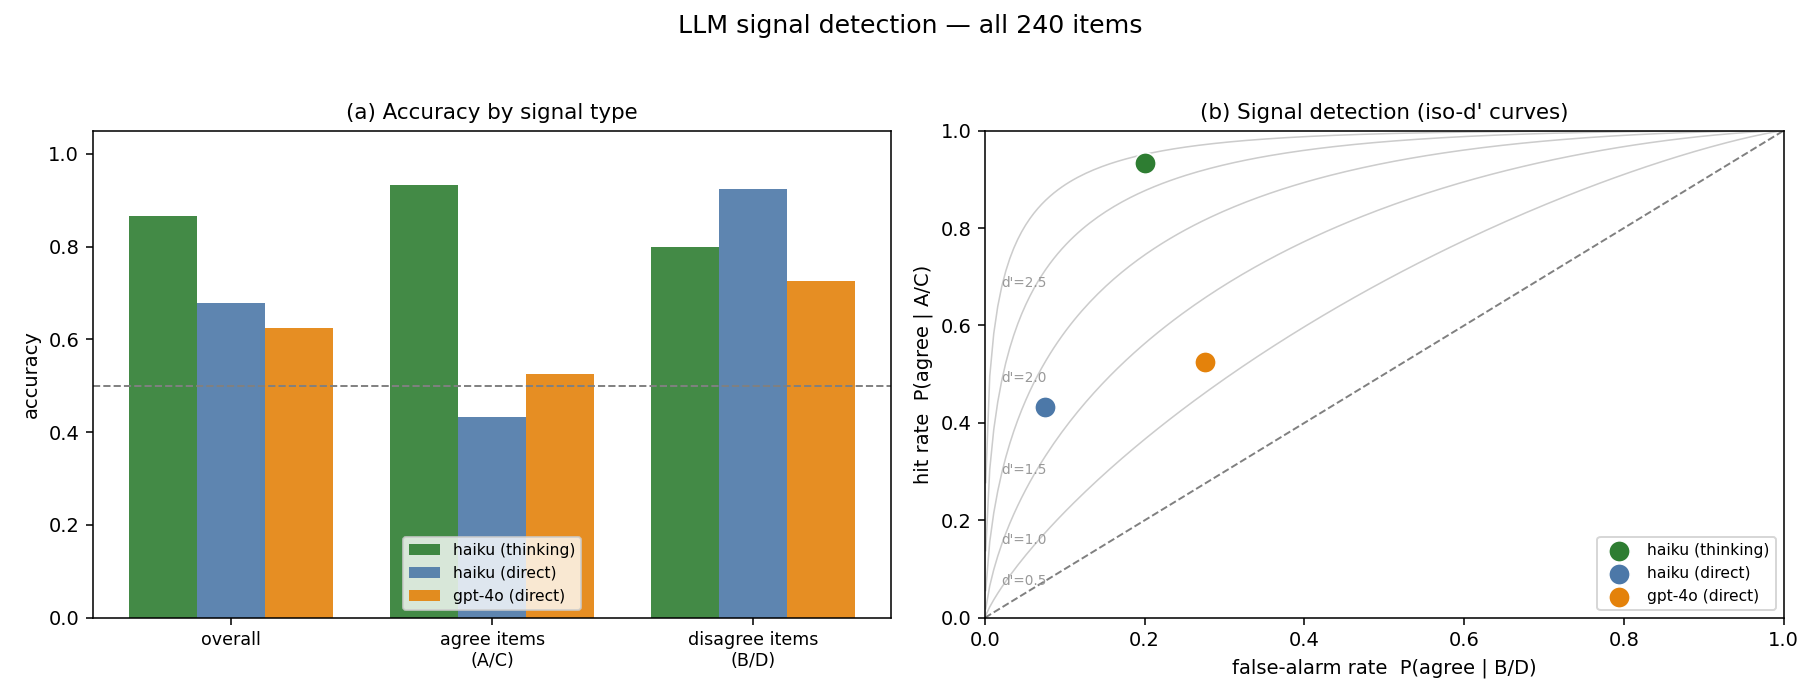
\includegraphics[width=\textwidth]{figs/llm_signal_detection.png}
  \caption{(a) Accuracy split by signal type: only the thinking regime clears chance on the
  agree-items (A/C). (b) The same data in ROC space with iso-$\dprime$ curves: \haiku{}-thinking
  sits near the top-left (high $\dprime$); the direct regimes are pulled down and toward the
  low-hit corner (conservative, disagree-biased).}
  \label{fig:signal}
\end{figure}

\begin{figure}[!htb]
  \centering
  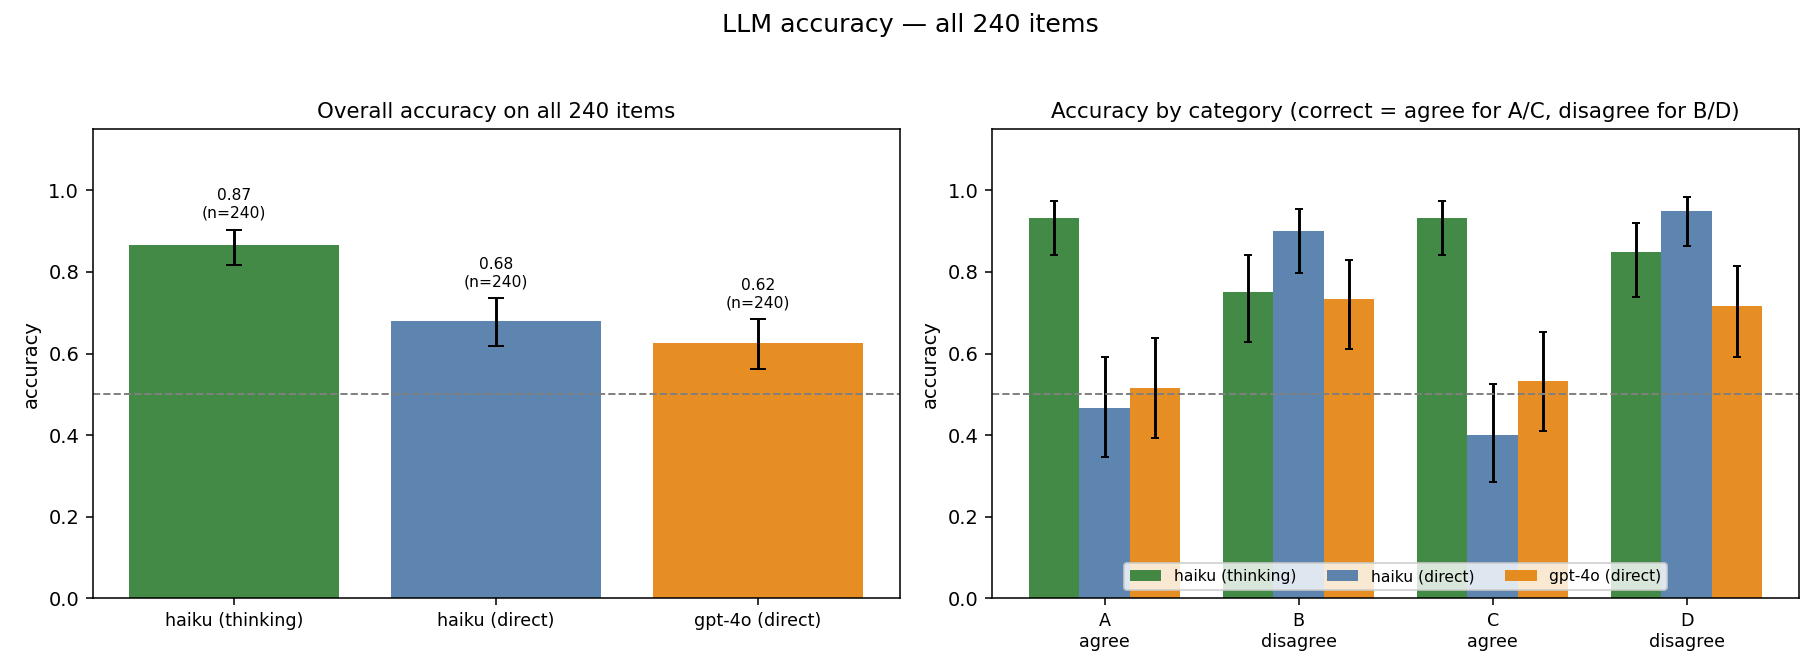
\includegraphics[width=\textwidth]{figs/llm_accuracy_overview.png}
  \caption{Overall accuracy per regime (left) and by stimulus category (right). The
  agree-items (A, C) are where the regimes separate: the direct models are at or below chance
  there while acing the disagree-items (B, D). Error bars/chance line as in the text.}
  \label{fig:overview}
\end{figure}

\subsection{Accuracy by misconception}
Figure~\ref{fig:bymisc} breaks accuracy down by the misconception present in the trace.
\haiku{}-thinking is high and flat across all six ($0.83$--$0.95$), though the sharper
per-probed-misconception analysis below shows this flatness hides real variation in
sensitivity. The direct regimes are lower and more jagged; \gpt{} even dips below chance on
the add-before-$\times$ items. For \haiku{}-thinking, paired (two-misconception) items are
\emph{not} harder than single-misconception ones, a contrast with the ideal-observer
baseline, whose confidence in the probed misconception drops on paired traces.

\begin{figure}[!htb]
  \centering
  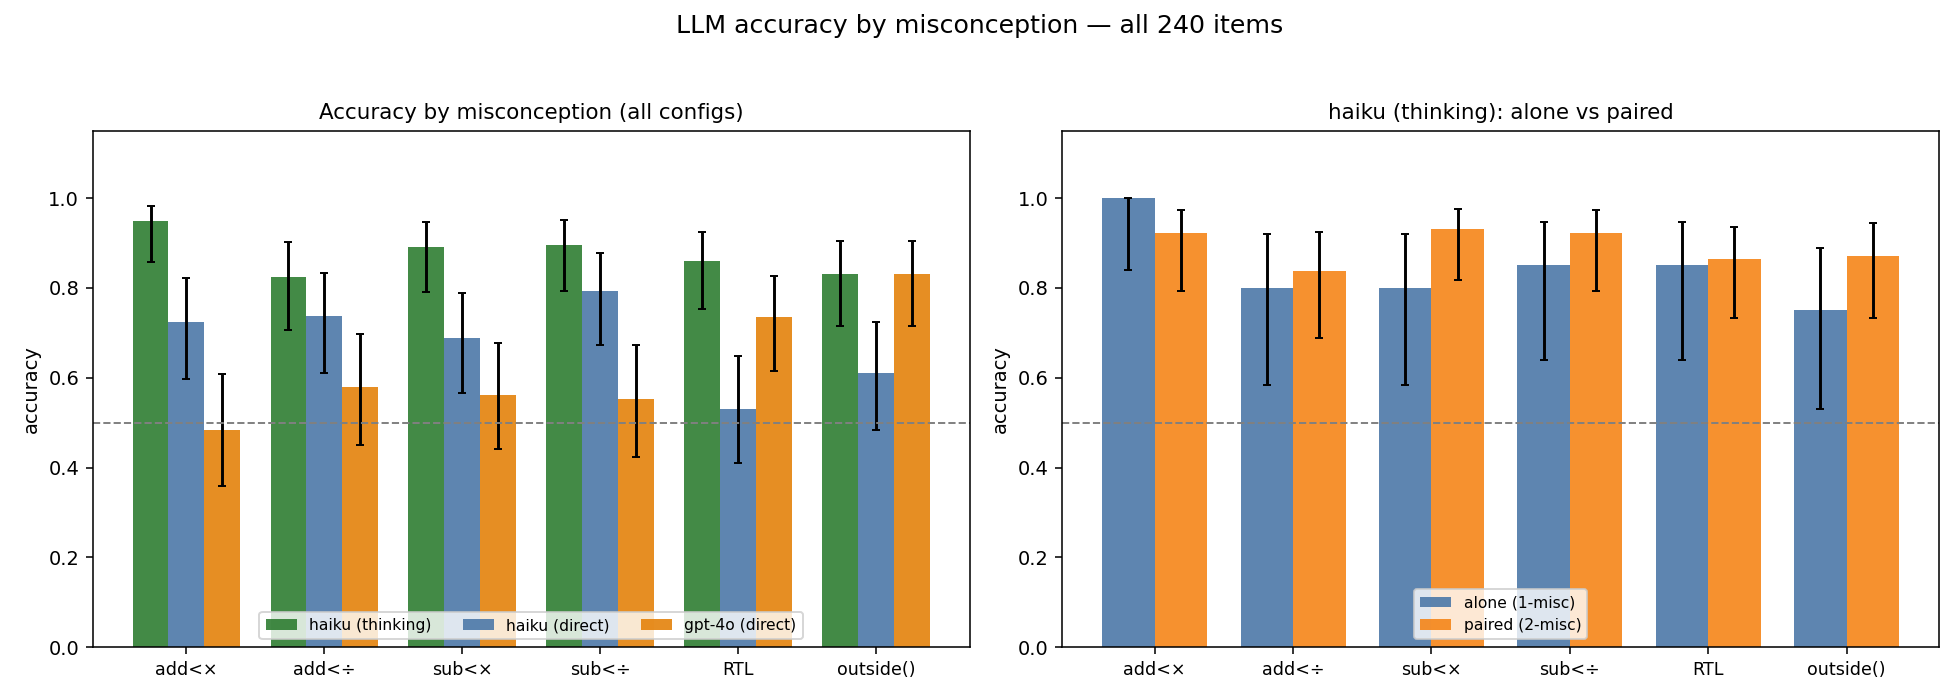
\includegraphics[width=\textwidth]{figs/llm_accuracy_by_misconception.png}
  \caption{Left: accuracy by misconception for all three regimes. Right: \haiku{}-thinking
  split into alone (one-misconception) vs.\ paired (two-misconception) items. The two are
  roughly balanced, i.e.\ the reasoning model does not degrade on paired traces.}
  \label{fig:bymisc}
\end{figure}

\subsection{Which misconceptions can each regime actually discriminate?}
Figure~\ref{fig:bymisc} groups trials by the misconception \emph{present} in the trace, which
mixes two different questions on foil items. A sharper cut groups trials by the misconception
\emph{named in the statement} (the probed one) and separates detection from rejection:
detection $=$ P(agree $\mid$ named \emph{and} present), from A items and C items where it is
the target; false alarm $=$ P(agree $\mid$ named but \emph{absent}), from B/D foil items. Each
probed misconception then gets its own $\dprime$ ($n = 20$ signal $+$ $20$ noise trials per
regime). Figure~\ref{fig:dprime} shows that the flat accuracy profile of
Figure~\ref{fig:bymisc} was hiding large variation.

\haiku{}-thinking's per-misconception $\dprime$ ranges from $1.64$ to $3.92$, and its two weak
spots are specific. For add-before-$\times$ the weakness is on the rejection side: when
``believes addition should be done before multiplication'' is named but absent, it wrongly
agrees $50\%$ of the time. For right-to-left it is on the detection side: it detects only
$0.75$ of genuinely present right-to-left errors, its lowest hit rate.

\haiku{}-direct cannot detect right-to-left at all ($\dprime = 0.00$; it agreed to a true
right-to-left statement once in 20 chances), and barely detects the bracket misconception
($\dprime = 0.36$). Without reasoning it discriminates only the four cross-precedence errors
($\dprime$ $1.16$--$2.21$), and even those under its strong disagree bias.

\gpt{} shows the \emph{reversed} profile, and this is the clearest surface-cue evidence in the
experiment: for right-to-left it agrees $80\%$ of the time when the statement is true and
$65\%$ when it is false ($\dprime = 0.46$); for the bracket misconception, $90\%$ vs.\ $75\%$
($\dprime = 0.61$). Its response tracks \emph{which statement type is named}, not what the
trace shows: it likes endorsing right-to-left and bracket statements and rejecting
cross-precedence ones, largely independent of the work. This is the BODMAS analog of the
numberlink pilot's ``path drawn $\Rightarrow$ say no'' rule.

\begin{figure}[!htb]
  \centering
  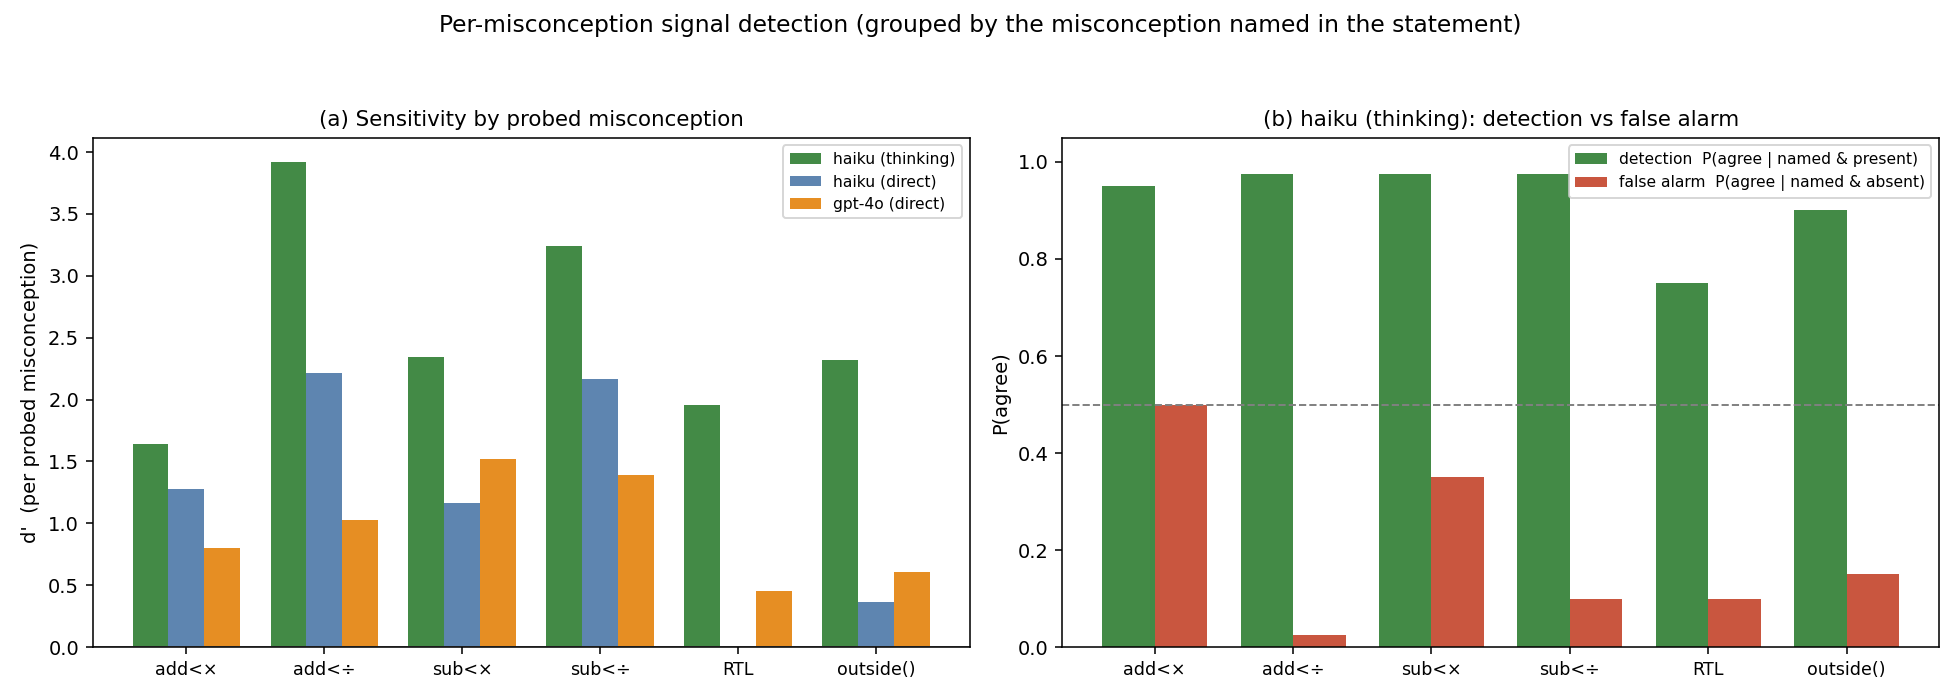
\includegraphics[width=\textwidth]{figs/llm_dprime_by_misconception.png}
  \caption{(a) Per-misconception $\dprime$, grouping trials by the misconception named in the
  statement. (b) The components for \haiku{}-thinking: detection rate vs.\ false-alarm rate per
  probed misconception. Its weak spots are add-before-$\times$ (false alarms) and right-to-left
  (misses).}
  \label{fig:dprime}
\end{figure}

\subsection{False alarms are structured: trace-driven near-misses vs.\ statement-driven endorsement}
Figure~\ref{fig:confusion} asks whether the models' false alarms (agreeing to a foil) are
random or structured, by crossing the misconception \emph{present} in the trace with the
absent foil \emph{named} in the statement.

The two regimes fail in qualitatively different ways. \haiku{}-thinking's rare false alarms
are \emph{row-structured}, i.e.\ driven by what is actually in the trace, and they are
near-miss confusions between behaviorally adjacent misconceptions: with add-before-$\div$
present it endorses ``add before $\times$'' at $0.67$; with sub-before-$\times$ present it
endorses ``add before $\times$'' at $0.67$; with sub-before-$\div$ present it endorses ``sub
before $\times$'' at $0.50$. In each case the falsely endorsed statement shares an operator
with the real error (the same low-priority operation fired early, or the same high-priority
operation deferred). The model saw something real in the work and matched it to a semantically
neighboring statement: partial reasoning, not noise.

The pooled direct regimes are instead \emph{column-structured}: the right-to-left and bracket
columns are hot ($0.25$--$0.58$) regardless of what is present. Their false alarms depend on
what is \emph{named}, not on what is \emph{shown}, confirming the statement-type cue from
Figure~\ref{fig:dprime}.

\begin{figure}[!htb]
  \centering
  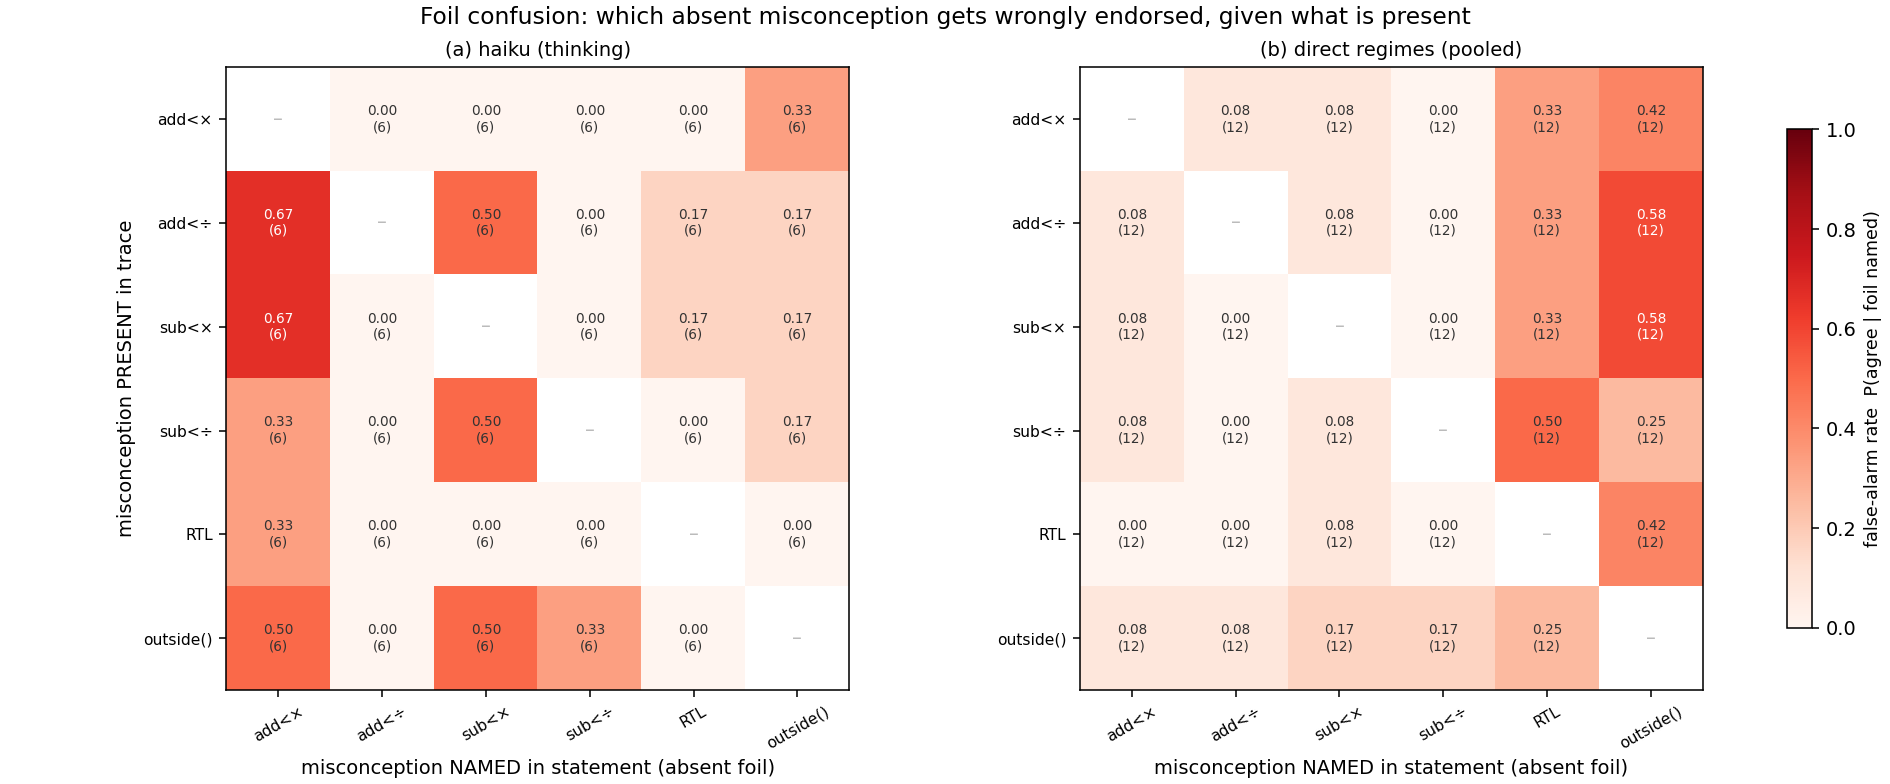
\includegraphics[width=\textwidth]{figs/llm_foil_confusion.png}
  \caption{False-alarm rate on foil trials, by the misconception present in the trace (rows)
  and the absent misconception named in the statement (columns); cell annotations give the rate
  and (n). (a) \haiku{}-thinking: row-structured near-miss confusions. (b) Direct regimes
  pooled: column-structured endorsement of right-to-left and bracket statements independent of
  the trace. Diagonal cells cannot occur (a named-and-present misconception is not a foil).}
  \label{fig:confusion}
\end{figure}

\subsection{Response style: how the direct models respond}
Figure~\ref{fig:response} shows the mechanism behind the bias. The direct regimes use the
6-point scale almost as a \emph{binary}: \haiku{}-direct places $74\%$ of its responses on
``Strongly Disagree'' and the rest near ``Strongly Agree,'' barely touching the middle; \gpt{}
is similar. \haiku{}-thinking uses the full graded scale. Overall agree-rates make the bias
quantitative: against a true agree-rate of $50\%$ (half the pool is agree-correct),
\haiku{}-thinking agrees $57\%$ of the time, \gpt{} $40\%$, and \haiku{}-direct only $25\%$.

\begin{figure}[!htb]
  \centering
  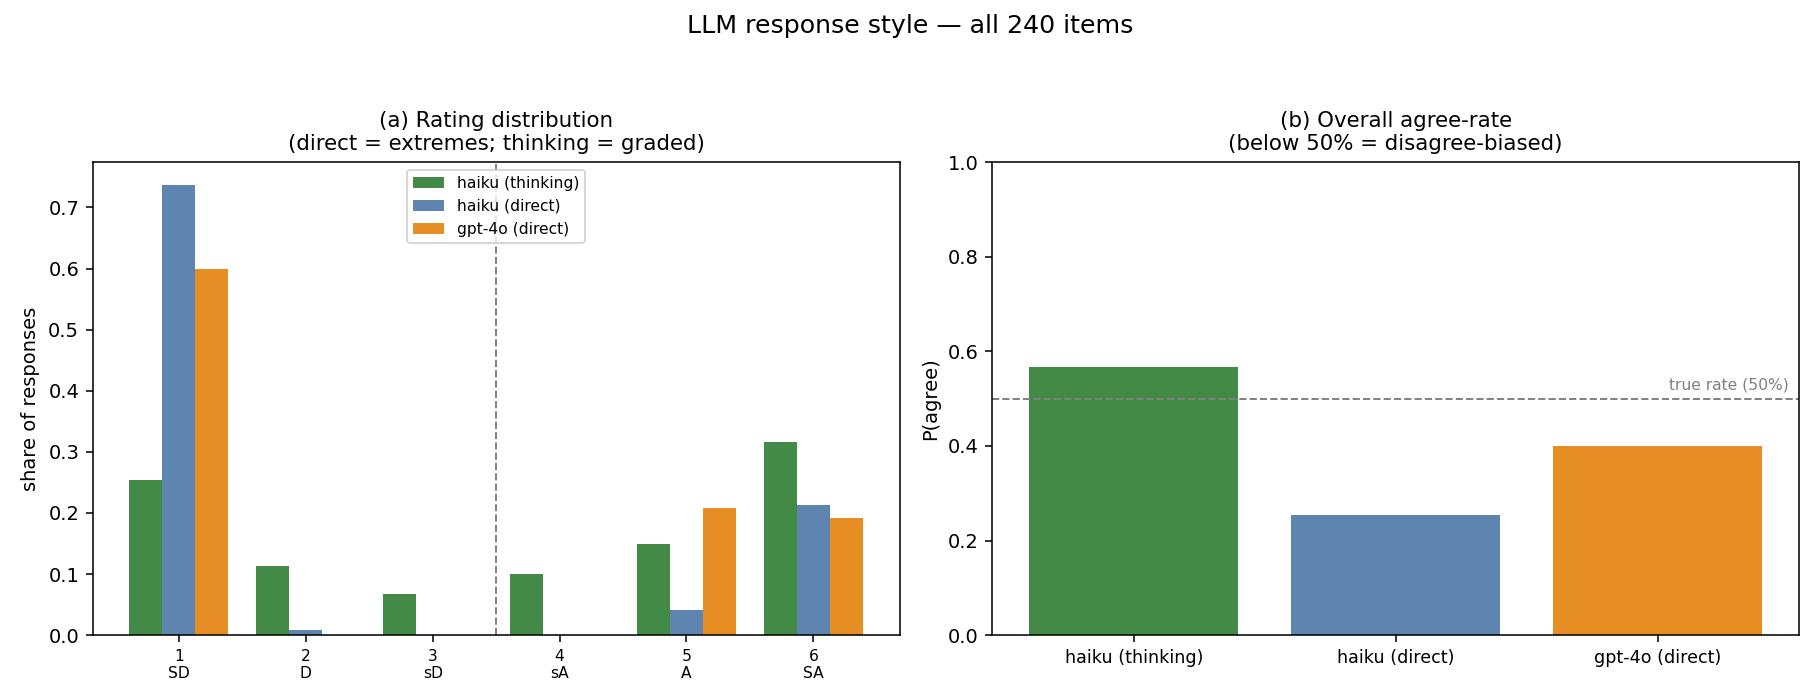
\includegraphics[width=\textwidth]{figs/llm_response_style.png}
  \caption{(a) Rating distribution per regime: the direct models pile on the extremes
  (especially ``Strongly Disagree''); thinking is graded. (b) Overall agree-rate vs.\ the true
  $50\%$: below $50\%$ indicates a disagree-bias.}
  \label{fig:response}
\end{figure}

\subsection{Thinking tokens as a reaction-time analog}
For the reasoning regime we treat thinking-token counts the way we treat human reaction time
(Figure~\ref{fig:tokens}). Two human-like patterns emerge. First, the harder \emph{direction}
costs more: disagree-items (ruling a foil out) take more thinking than agree-items (median
$732$ vs.\ $651$ tokens; $p = .004$), echoing ``establishing that something is \emph{not} the
case takes longer.'' Second, errors are slow: incorrect answers take far more thinking than
correct ones (median $1126$ vs.\ $672$ tokens; $p < 10^{-3}$), and accuracy falls monotonically
across token quartiles ($0.93 \to 0.72$), the ``think longer, still fail'' signature of a
search budget running out. Thinking tokens do \emph{not} scale with the number of
misconceptions ($\rho = 0.05$, n.s.), as expected: unlike the numberlink grid-size axis, our
items have no strong built-in difficulty gradient (all are four-operator expressions).

\begin{figure}[!htb]
  \centering
  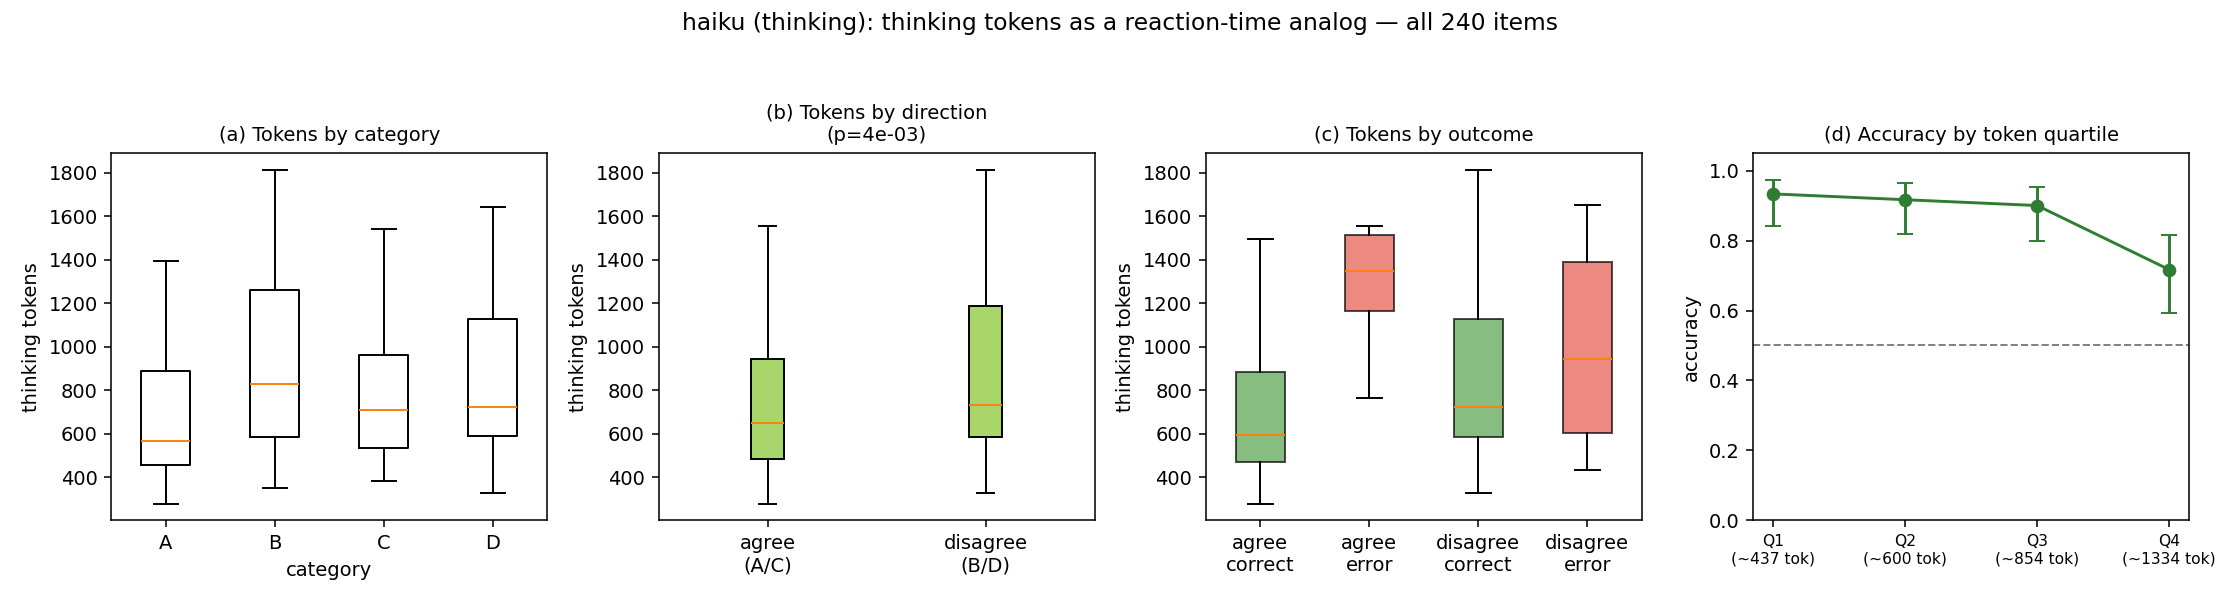
\includegraphics[width=\textwidth]{figs/llm_thinking_tokens.png}
  \caption{\haiku{} (thinking), $n = 240$. (a) Tokens by category. (b) Tokens by direction:
  disagree-items cost more than agree-items. (c) Tokens by outcome: errors are slow in both
  directions. (d) Accuracy by thinking-token quartile: more thinking marks harder items.}
  \label{fig:tokens}
\end{figure}

\subsection{Confidence, and the partial-explanation nuance}
We take the Likert magnitude $|\text{rating}-3.5|$ as a confidence signal
(Figure~\ref{fig:confidence}a). It is calibrated \emph{only} for the reasoning regime:
\haiku{}-thinking is more confident when correct than when wrong (AUC $= 0.79$), while both
direct regimes are uniformly over-confident regardless of correctness (AUC $\approx 0.50$),
consistent with their near-binary, unreflective responding. A reasoning trace apparently gives
the model something real to be uncertain about.

Figure~\ref{fig:confidence}b tests whether the models perceive that a category-C statement is a
\emph{partial} explanation (it names one of two present misconceptions). Among the items it
agreed with, \haiku{}-thinking rates single-misconception A items at $5.73$ but partial-match C
items at only $5.32$, a clear, confidence-interval-separated gap: it moderates its agreement
when the statement leaves a second error unexplained. \haiku{}-direct shows a smaller gap and
\gpt{} shows none ($5.52$ vs.\ $5.50$), i.e.\ only the reasoning model registers the
distinction.

\begin{figure}[!htb]
  \centering
  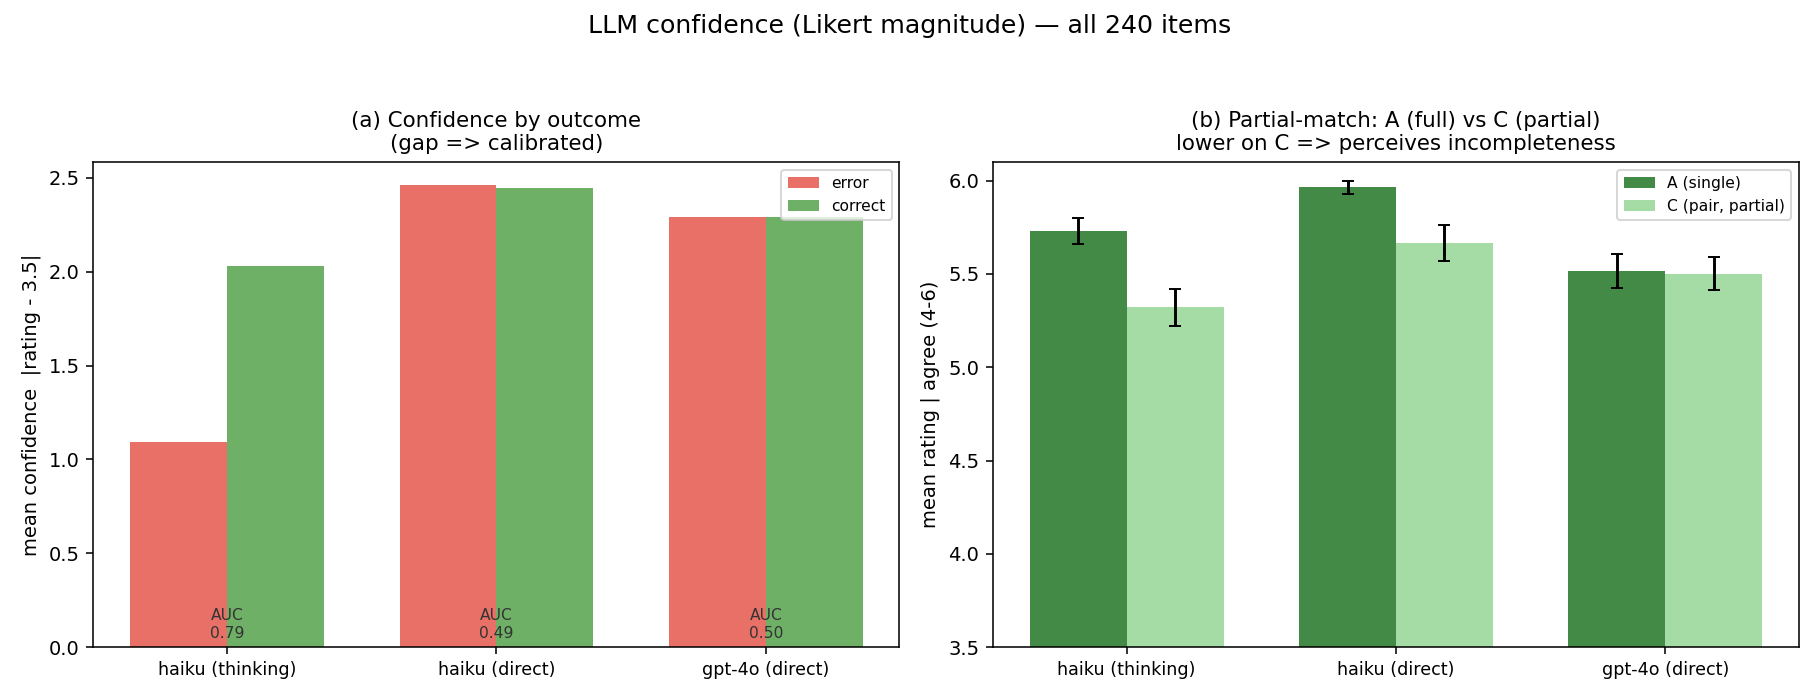
\includegraphics[width=\textwidth]{figs/llm_confidence.png}
  \caption{(a) Mean confidence ($|\text{rating}-3.5|$) by outcome: only \haiku{}-thinking shows
  a correct/error gap (AUC $0.79$ vs.\ $\approx 0.50$). (b) Among agree responses, mean rating
  on single-misconception A vs.\ partial-match C items: a lower C rating means the model
  perceives the incompleteness.}
  \label{fig:confidence}
\end{figure}

\subsection{Where the evidence sits: early vs.\ late errors in category C}
In a category-C trace both misconceptions leave errors, at different steps, and
\texttt{which\_target} records whether the \emph{named} misconception's error appears first or
later than its partner's (balanced $30/30$ per regime by construction). Figure~\ref{fig:position}
asks whether detection depends on where the evidence sits in the work.

Only the reasoning model shows a position effect, and it appears most clearly in the graded
measure: \haiku{}-thinking's accuracy dips slightly when the named error comes later ($0.97 \to
0.90$), but its mean rating drops from $5.50$ to $4.80$. It still finds a late-buried error,
yet endorses the statement less strongly, a primacy-like weighting of early evidence familiar
from human reading. The direct regimes show no consistent position effect (\haiku{}-direct
$0.37$ vs.\ $0.43$; \gpt{} $0.57$ vs.\ $0.50$, both within noise), consistent with their not
stepping through the trace at all. Because the human experiment samples exactly this
first/second contrast (three of each per participant), this panel is directly comparable to
the human data once collected.

\begin{figure}[!htb]
  \centering
  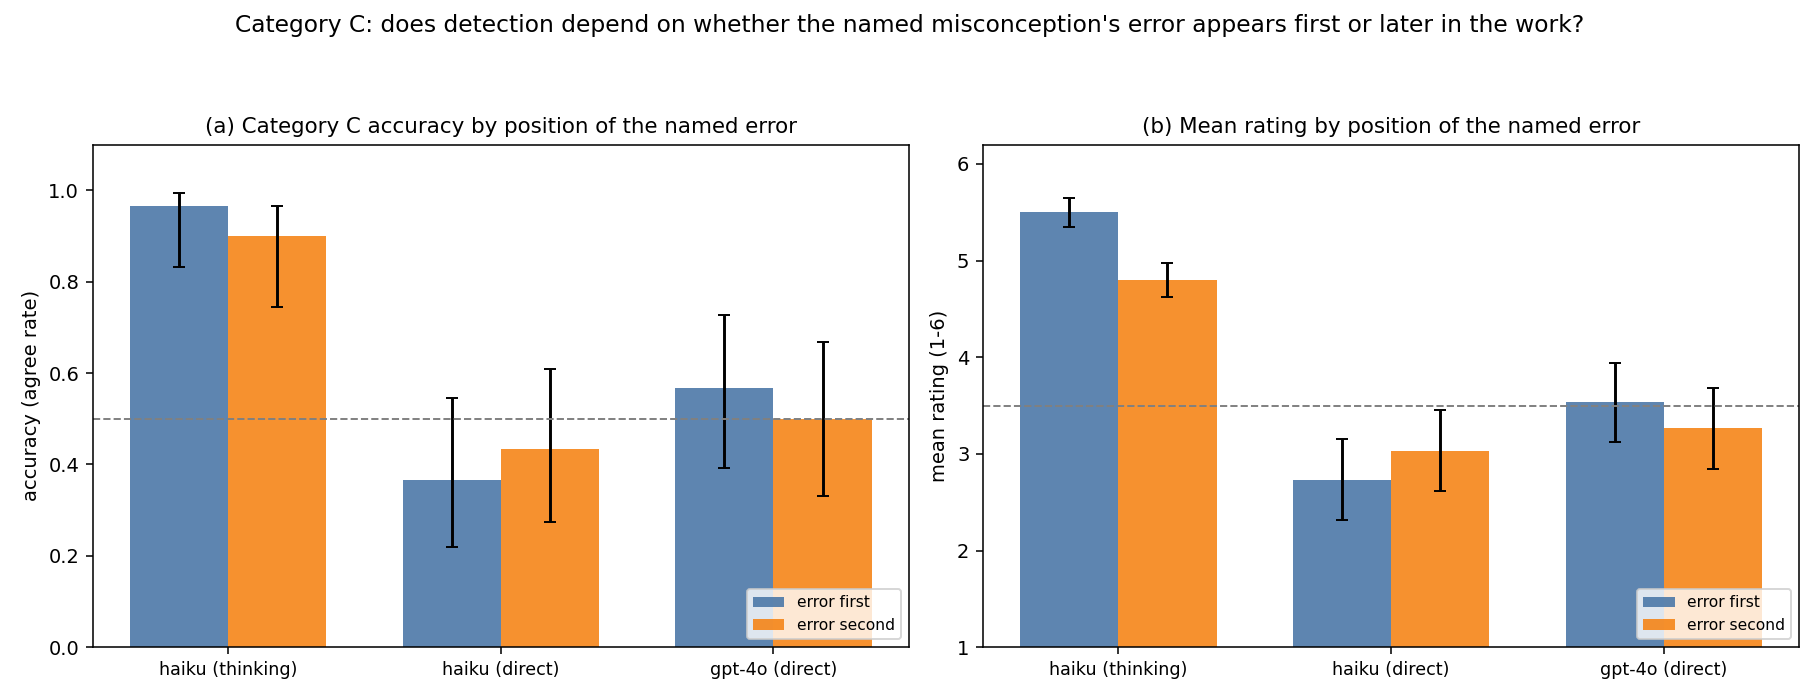
\includegraphics[width=\textwidth]{figs/llm_error_position.png}
  \caption{Category C, by whether the named misconception's error appears first or later in
  the student's work ($n = 30$ per bar). (a) Accuracy (agree is correct in C). (b) Mean rating:
  \haiku{}-thinking endorses the statement less strongly when its evidence appears later
  ($5.50 \to 4.80$); the direct regimes show no consistent position effect.}
  \label{fig:position}
\end{figure}

\subsection{Cost and latency}
The reasoning regime is the only one with a real cost (Table~\ref{tab:cost}): $\sim$13$\times$
the latency and $\sim$220$\times$ the output tokens of its direct counterpart. That is the
price of the only regime that can actually do the task.

\begin{table}[!htb]
\centering\small
\caption{Operational profile per regime (240 items each). Latency is the median per call;
tokens are totals over the regime.}
\label{tab:cost}
\begin{tabular}{@{}lrrr@{}}
\toprule
regime & median latency & total prompt tokens & total output tokens \\
\midrule
\gpt{} (direct)      & 0.6\,s  & 77k  & 1.3k \\
\haiku{} (direct)    & 1.0\,s  & 114k & 2.2k \\
\haiku{} (thinking)  & 13.0\,s & 121k & 478k (of which 195k reasoning) \\
\bottomrule
\end{tabular}
\end{table}

\section{Discussion}
Without reasoning, both models default to a conservative ``disagree'' and use the scale as a
near-binary; they retain partial sensitivity but are dominated by response bias. The
per-misconception and confusion analyses localize what that bias is made of: \gpt{}'s
responses track the \emph{statement type} (endorsing right-to-left and bracket claims,
rejecting cross-precedence ones, largely independent of the trace), and the direct regimes'
false alarms are column-structured accordingly. Extended reasoning transforms \haiku{}: it
discriminates ($\dprime = 2.34$), drops the bias, uses the graded scale, becomes
confidence-calibrated, and registers the partial-explanation structure of the two-misconception
items. Its remaining errors look like \emph{partial reasoning} rather than noise: false alarms
are near-miss confusions between operator-adjacent misconceptions, and statements whose
evidence appears later in the work are endorsed less strongly. \gpt{}, unable to reason here,
stays biased and oblivious. Thinking tokens carry human-reaction-time-like structure (harder
direction and errors cost more). The natural next step is the three-way comparison against
human participants and the Bayesian ideal observer over the same 240-item pool: are the
misconceptions and categories that are hard for people the same ones that are hard for the
reasoning model and, in principle, for an ideal reasoner? The human-side dataset drops into
this analysis by construction.

\end{document}
